% Made up for the tikra benchmark.
\usetikzlibrary{decorations.footprints}
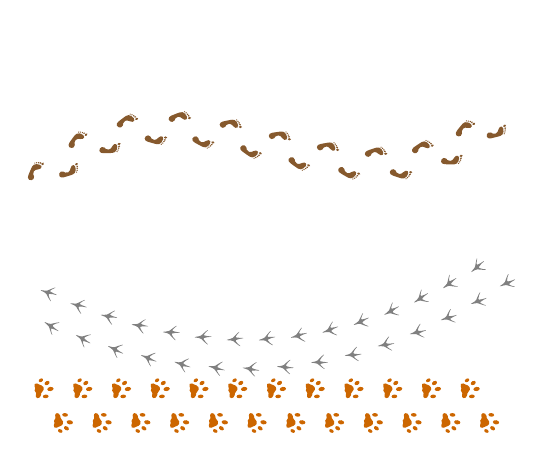
\begin{tikzpicture}
  \fill[decorate, decoration={footprints, foot length=8pt, stride length=18pt, foot of=human}, brown!70!black]
    (0,0) .. controls (2,2) and (4,-1) .. (6,1);
  \fill[decorate, decoration={footprints, foot length=6pt, stride length=12pt, foot of=bird}, gray]
    (0,-1.5) to[bend right] (6,-1);
  \fill[decorate, decoration={footprints, foot length=7pt, stride length=14pt, foot of=felis silvestris}, orange!80!black]
    (0,-2.8) -- (6,-2.8);
\end{tikzpicture}
